\documentclass[10pt,ignorenonframetext,,aspectratio=149]{beamer}
\setbeamertemplate{caption}[numbered]
\setbeamertemplate{caption label separator}{: }
\setbeamercolor{caption name}{fg=normal text.fg}
\usepackage{lmodern}
\usepackage{amssymb,amsmath}
\usepackage{ifxetex,ifluatex}
\usepackage{fixltx2e} % provides \textsubscript
\ifnum 0\ifxetex 1\fi\ifluatex 1\fi=0 % if pdftex
  \usepackage[T1]{fontenc}
  \usepackage[utf8]{inputenc}
\else % if luatex or xelatex
  \ifxetex
    \usepackage{mathspec}
  \else
    \usepackage{fontspec}
  \fi
  \defaultfontfeatures{Ligatures=TeX,Scale=MatchLowercase}
  \newcommand{\euro}{€}
\fi
% use upquote if available, for straight quotes in verbatim environments
\IfFileExists{upquote.sty}{\usepackage{upquote}}{}
% use microtype if available
\IfFileExists{microtype.sty}{%
\usepackage{microtype}
\UseMicrotypeSet[protrusion]{basicmath} % disable protrusion for tt fonts
}{}
\usepackage{color}
\usepackage{fancyvrb}
\newcommand{\VerbBar}{|}
\newcommand{\VERB}{\Verb[commandchars=\\\{\}]}
\DefineVerbatimEnvironment{Highlighting}{Verbatim}{commandchars=\\\{\}}
% Add ',fontsize=\small' for more characters per line
\usepackage{framed}
\definecolor{shadecolor}{RGB}{248,248,248}
\newenvironment{Shaded}{\begin{snugshade}}{\end{snugshade}}
\newcommand{\AlertTok}[1]{\textcolor[rgb]{0.94,0.16,0.16}{#1}}
\newcommand{\AnnotationTok}[1]{\textcolor[rgb]{0.56,0.35,0.01}{\textbf{\textit{#1}}}}
\newcommand{\AttributeTok}[1]{\textcolor[rgb]{0.77,0.63,0.00}{#1}}
\newcommand{\BaseNTok}[1]{\textcolor[rgb]{0.00,0.00,0.81}{#1}}
\newcommand{\BuiltInTok}[1]{#1}
\newcommand{\CharTok}[1]{\textcolor[rgb]{0.31,0.60,0.02}{#1}}
\newcommand{\CommentTok}[1]{\textcolor[rgb]{0.56,0.35,0.01}{\textit{#1}}}
\newcommand{\CommentVarTok}[1]{\textcolor[rgb]{0.56,0.35,0.01}{\textbf{\textit{#1}}}}
\newcommand{\ConstantTok}[1]{\textcolor[rgb]{0.00,0.00,0.00}{#1}}
\newcommand{\ControlFlowTok}[1]{\textcolor[rgb]{0.13,0.29,0.53}{\textbf{#1}}}
\newcommand{\DataTypeTok}[1]{\textcolor[rgb]{0.13,0.29,0.53}{#1}}
\newcommand{\DecValTok}[1]{\textcolor[rgb]{0.00,0.00,0.81}{#1}}
\newcommand{\DocumentationTok}[1]{\textcolor[rgb]{0.56,0.35,0.01}{\textbf{\textit{#1}}}}
\newcommand{\ErrorTok}[1]{\textcolor[rgb]{0.64,0.00,0.00}{\textbf{#1}}}
\newcommand{\ExtensionTok}[1]{#1}
\newcommand{\FloatTok}[1]{\textcolor[rgb]{0.00,0.00,0.81}{#1}}
\newcommand{\FunctionTok}[1]{\textcolor[rgb]{0.00,0.00,0.00}{#1}}
\newcommand{\ImportTok}[1]{#1}
\newcommand{\InformationTok}[1]{\textcolor[rgb]{0.56,0.35,0.01}{\textbf{\textit{#1}}}}
\newcommand{\KeywordTok}[1]{\textcolor[rgb]{0.13,0.29,0.53}{\textbf{#1}}}
\newcommand{\NormalTok}[1]{#1}
\newcommand{\OperatorTok}[1]{\textcolor[rgb]{0.81,0.36,0.00}{\textbf{#1}}}
\newcommand{\OtherTok}[1]{\textcolor[rgb]{0.56,0.35,0.01}{#1}}
\newcommand{\PreprocessorTok}[1]{\textcolor[rgb]{0.56,0.35,0.01}{\textit{#1}}}
\newcommand{\RegionMarkerTok}[1]{#1}
\newcommand{\SpecialCharTok}[1]{\textcolor[rgb]{0.00,0.00,0.00}{#1}}
\newcommand{\SpecialStringTok}[1]{\textcolor[rgb]{0.31,0.60,0.02}{#1}}
\newcommand{\StringTok}[1]{\textcolor[rgb]{0.31,0.60,0.02}{#1}}
\newcommand{\VariableTok}[1]{\textcolor[rgb]{0.00,0.00,0.00}{#1}}
\newcommand{\VerbatimStringTok}[1]{\textcolor[rgb]{0.31,0.60,0.02}{#1}}
\newcommand{\WarningTok}[1]{\textcolor[rgb]{0.56,0.35,0.01}{\textbf{\textit{#1}}}}
\usepackage{graphicx,grffile}
\makeatletter
\def\maxwidth{\ifdim\Gin@nat@width>\linewidth\linewidth\else\Gin@nat@width\fi}
\def\maxheight{\ifdim\Gin@nat@height>\textheight0.8\textheight\else\Gin@nat@height\fi}
\makeatother
% Scale images if necessary, so that they will not overflow the page
% margins by default, and it is still possible to overwrite the defaults
% using explicit options in \includegraphics[width, height, ...]{}
\setkeys{Gin}{width=\maxwidth,height=\maxheight,keepaspectratio}

% Comment these out if you don't want a slide with just the
% part/section/subsection/subsubsection title:
\AtBeginPart{
  \let\insertpartnumber\relax
  \let\partname\relax
  \frame{\partpage}
}
\AtBeginSection{
  \let\insertsectionnumber\relax
  \let\sectionname\relax
  \frame{\sectionpage}
}
\AtBeginSubsection{
  \let\insertsubsectionnumber\relax
  \let\subsectionname\relax
  \frame{\subsectionpage}
}

\setlength{\emergencystretch}{3em}  % prevent overfull lines
\providecommand{\tightlist}{%
  \setlength{\itemsep}{0pt}\setlength{\parskip}{0pt}}
\setcounter{secnumdepth}{0}

\title{ACT-11302 Calculo Actuarial III}
\subtitle{Sesion 03 - Inferencia en distribuciones tipo mixtas - Parte 1}
\author{Juan Carlos Martinez-Ovando}
\date{}

%% Here's everything I added.
%%--------------------------

\usepackage{graphicx}
\usepackage{rotating}
%\setbeamertemplate{caption}[numbered]
\usepackage{hyperref}
\usepackage{caption}
\usepackage[normalem]{ulem}
%\mode<presentation>
\usepackage{wasysym}
%\usepackage{amsmath}


% Get rid of navigation symbols.
%-------------------------------
\setbeamertemplate{navigation symbols}{}

% Optional institute tags and titlegraphic.
% Do feel free to change the titlegraphic if you don't want it as a Markdown field.
%----------------------------------------------------------------------------------
\institute{Departamento Academico de Actuaria y Seguros}

% \titlegraphic{\includegraphics[width=0.3\paperwidth]{\string~/Dropbox/teaching/clemson-academic.png}} % <-- if you want to know what this looks like without it as a Markdown field. 
% -----------------------------------------------------------------------------------------------------
\titlegraphic{
\includegraphics[width=0.3\paperwidth]{\string~/svm-r-sources/ITAM2016.png}}

% Some additional title page adjustments.
%----------------------------------------
\setbeamertemplate{title page}[empty]
%\date{}
\setbeamerfont{subtitle}{size=\small}

\setbeamercovered{transparent}

% Some optional colors. Change or add as you see fit.
%---------------------------------------------------
\definecolor{clemsonpurple}{HTML}{522D80}
% \definecolor{clemsonorange}{HTML}{EA6A20}
 \definecolor{clemsonorange}{HTML}{F66733}
\definecolor{uiucblue}{HTML}{003C7D}
\definecolor{uiucorange}{HTML}{F47F24}


% Some optional color adjustments to Beamer. Change as you see fit.
%------------------------------------------------------------------
\setbeamercolor{frametitle}{fg=clemsonpurple,bg=white}
\setbeamercolor{title}{fg=clemsonpurple,bg=white}
\setbeamercolor{local structure}{fg=clemsonpurple}
\setbeamercolor{section in toc}{fg=clemsonpurple,bg=white}
% \setbeamercolor{subsection in toc}{fg=clemsonorange,bg=white}
\setbeamercolor{footline}{fg=clemsonpurple!50, bg=white}
\setbeamercolor{block title}{fg=clemsonorange,bg=white}


\let\Tiny=\tiny


% Sections and subsections should not get their own damn slide.
%--------------------------------------------------------------
\AtBeginPart{}
\AtBeginSection{}
\AtBeginSubsection{}
\AtBeginSubsubsection{}

% Suppress some of Markdown's weird default vertical spacing.
%------------------------------------------------------------
\setlength{\emergencystretch}{0em}  % prevent overfull lines
\setlength{\parskip}{0pt}


% Allow for those simple two-tone footlines I like. 
% Edit the colors as you see fit.
%--------------------------------------------------
\defbeamertemplate*{footline}{my footline}{%
    \ifnum\insertpagenumber=1
    \hbox{%
        \begin{beamercolorbox}[wd=\paperwidth,ht=.8ex,dp=1ex,center]{}%
      % empty environment to raise height
        \end{beamercolorbox}%
    }%
    \vskip0pt%
    \else%
        \Tiny{%
            \hfill%
		\vspace*{1pt}%
            \insertframenumber/\inserttotalframenumber \hspace*{0.1cm}%
            \newline%
            \color{clemsonpurple}{\rule{\paperwidth}{0.4mm}}\newline%
            \color{clemsonorange}{\rule{\paperwidth}{.4mm}}%
        }%
    \fi%
}

% Various cosmetic things, though I must confess I forget what exactly these do and why I included them.
%-------------------------------------------------------------------------------------------------------
\setbeamercolor{structure}{fg=blue}
\setbeamercolor{local structure}{parent=structure}
\setbeamercolor{item projected}{parent=item,use=item,fg=clemsonpurple,bg=white}
\setbeamercolor{enumerate item}{parent=item}

% Adjust some item elements. More cosmetic things.
%-------------------------------------------------
\setbeamertemplate{itemize item}{\color{clemsonpurple}$\bullet$}
\setbeamertemplate{itemize subitem}{\color{clemsonpurple}\scriptsize{$\bullet$}}
\setbeamertemplate{itemize/enumerate body end}{\vspace{.6\baselineskip}} % So I'm less inclined to use \medskip and \bigskip in Markdown.

% Automatically center images
% ---------------------------
% Note: this is for ![](image.png) images
% Use "fig.align = "center" for R chunks

\usepackage{etoolbox}

\AtBeginDocument{%
  \letcs\oig{@orig\string\includegraphics}%
  \renewcommand<>\includegraphics[2][]{%
    \only#3{%
      {\centering\oig[{#1}]{#2}\par}%
    }%
  }%
}

% I think I've moved to xelatex now. Here's some stuff for that.
% --------------------------------------------------------------
% I could customize/generalize this more but the truth is it works for my circumstances.

\ifxetex
\setbeamerfont{title}{family=\fontspec{serif}}
\setbeamerfont{frametitle}{family=\fontspec{serif}}
\usepackage[font=small,skip=0pt]{caption}
 \else
 \fi

% Okay, and begin the actual document...

\begin{document}
\frame{\titlepage}

\begin{frame}

\end{frame}

\begin{frame}[fragile]{Objetivo}
\protect\hypertarget{objetivo}{}

\begin{itemize}
\item
  Estudiar las implicaciones de la \texttt{propiedad\ de\ separacion} en
  el proceso inferencia tipo mixto.
\item
  Incorporar \texttt{datos} en el proceso inferencial.
\item
  Incorporar \texttt{datos} e \texttt{informacion\ complementaria} en el
  proceso inferencial.
\end{itemize}

\end{frame}

\begin{frame}{Preambulo}
\protect\hypertarget{preambulo}{}

Seguimos considerando la clase de modelos tipo mixto con soporte en
\(\mathcal{X}=\{0\}\cup (0,\infty)\), y ``densidad'' dada por \[
f(x|\theta_0,\theta_c)=\theta_0 \mathbb{I}(x=0)+(1-\theta_0)\theta_c\exp\{-\theta_c x\}\mathbb{I}(x>0).
\] Como vimos, esta clase de modelos puede verse como una composicion
considerando la variable auxiliar \[
Z=\begin{cases}
1, \text{ si } x=0 \text{, con probabilidad } \theta_0,\\
0, \text{ si } x>0 \text{, con probabilidad } (1-\theta_0).\\
\end{cases}
\]

\end{frame}

\begin{frame}[fragile]{Problema inferencial}
\protect\hypertarget{problema-inferencial}{}

Si consideramos un conjunto de \texttt{datos} dado por una coleccion de
\(J\) observaciones/polizas que toman valores en \(\mathcal{X}\),
digamos \[
\text{datos}=\{x_1,\ldots,x_J\},
\] tendremos el \textbf{objetivo} de encontrar los valores de \[
\theta_0\text{ y }\theta_c,
\] que \textbf{sean mas compatibles con los datos}.

\begin{quote}
\textcolor{blue}{Recordemos que como $x_i\in\mathcal{X}$, esperaremos que varios $x_i$s compartan el valor $0$.}
\end{quote}

\end{frame}

\begin{frame}[fragile]{Datos}
\protect\hypertarget{datos}{}

Consideremos los datos reales de la empresa \textbf{AllState} de un
portafolio de seguros de autos.

Cargamos los datos desde un repositorio en GitHUb (en este caso, el
repositorio de datos de nuestro curso, referido como
\texttt{JCMO-ITAM/Data4Analysis}). Para esto, empleamos en RStudio el
paquete \texttt{repmis}. El diccionario de datos se encuentra en el
mismo repositorio.

\begin{verbatim}
if(!require("repmis")){install.packages("repmis")}
library("repmis")

data <- source_data("https://github.com/JCMO-ITAM/Data4Analysis/...
        blob/master/d4a_allstateclaim_data.csv?raw=true")
\end{verbatim}

\end{frame}

\begin{frame}[fragile]{Resumen}
\protect\hypertarget{resumen}{}

Los \texttt{datos} incluyen las siguientes variables:

\begin{verbatim}
## Loading required package: repmis
\end{verbatim}

\begin{verbatim}
## Downloading data from: https://github.com/JCMO-ITAM/Data4Analysis/blob/master/d4a_allstateclaim_data.csv?raw=true
\end{verbatim}

\begin{verbatim}
## SHA-1 hash of the downloaded data file is:
## f99c63d65351dd1ff9e67aa3c66c94f5d9139f22
\end{verbatim}

\begin{verbatim}
## [1] "Household_ID"  "Vehicle"       "Calendar_Year" "Model_Year"   
## [5] "Blind_Make"    "Claim_Amount"
\end{verbatim}

La variable \texttt{Claim\_Amount} representa el monto de reclamo
individual, nuestros valores \(x_i\).

Los casos \texttt{Claim\_Amount==0} representan no siniestro en la
poliza correspondiente.

\(J\) es el numero de polizas en los \texttt{datos}, y \(n\) es el
numero de polizas con no siniestro.

\begin{verbatim}
## [1] 330065
\end{verbatim}

\begin{verbatim}
## [1] 327064
\end{verbatim}

\end{frame}

\begin{frame}[fragile]{Verosimilitud}
\protect\hypertarget{verosimilitud}{}

La funcion de verosimilitud para \((\theta_0,\theta_c)\) con base en los
datos es (bajo el supuesto \texttt{iid}), \begin{eqnarray}
lik(\theta_0,\theta_c|\text{datos}) 
& = &
\prod_{i=1}^{J}f(x_i|\theta_0,\theta_c) \nonumber \\
& = &
\prod_{x_i:x_i=1}^{J}\theta_0 \times \prod_{x_i:x_i>0}(1-\theta_0)\theta_c\exp\{-\theta_c x_i\} \nonumber \\
& = &
\theta_0^{n_0} \times (1-\theta_0)^{J-n_0}\theta_c^{J-n_0}\exp\{-\theta_c \sum_{x_i:x_i>0}x_i\}, \nonumber
\end{eqnarray} donde \[
n_0=\#\{ x_i: x_i=0\}.
\]

\end{frame}

\begin{frame}[fragile]{Comentarios}
\protect\hypertarget{comentarios}{}

\begin{enumerate}
\item
  Noten que el componente
  \[\theta_0^{n_0} \times (1-\theta_0)^{J-n_0},\] resume la informacion
  en los datos para \(\theta_0\).
\item
  Noten que el componente
  \[\theta_c^{J-n_0}\exp\left\{-\theta_c \sum_{x_i:x_i>0}x_i\right\},\]
  resume la informacion para \(\theta_c\).
\item
  Ambas informacion son \texttt{separadas} pero \texttt{no\ ajenas}. Por
  esto, podemos hacer inferencia sobre \(\theta_0\) y \(\theta_c\) por
  \texttt{separado}.
\end{enumerate}

\end{frame}

\begin{frame}[fragile]{Maxima verosimilitud I}
\protect\hypertarget{maxima-verosimilitud-i}{}

Encontrar el EMV para \(\theta_0\) con base en los \texttt{datos} es
relativamente simple, es dado por \begin{eqnarray}
  \theta_0^{*}
  & = &
  \arg\max_{(0,1)} \theta_0^{n_0} \times (1-\theta_0)^{J-n_0} \nonumber \\
  & = &
  \frac{n_0}{J}. \nonumber
\end{eqnarray}

En el caso de los datos \textbf{AllState} es

\begin{Shaded}
\begin{Highlighting}[]
\NormalTok{theta0_star <-}\StringTok{ }\NormalTok{n0}\OperatorTok{/}\NormalTok{J}
\NormalTok{theta0_star}
\end{Highlighting}
\end{Shaded}

\begin{verbatim}
## [1] 0.9909079
\end{verbatim}

\end{frame}

\begin{frame}{Error epistemico I}
\protect\hypertarget{error-epistemico-i}{}

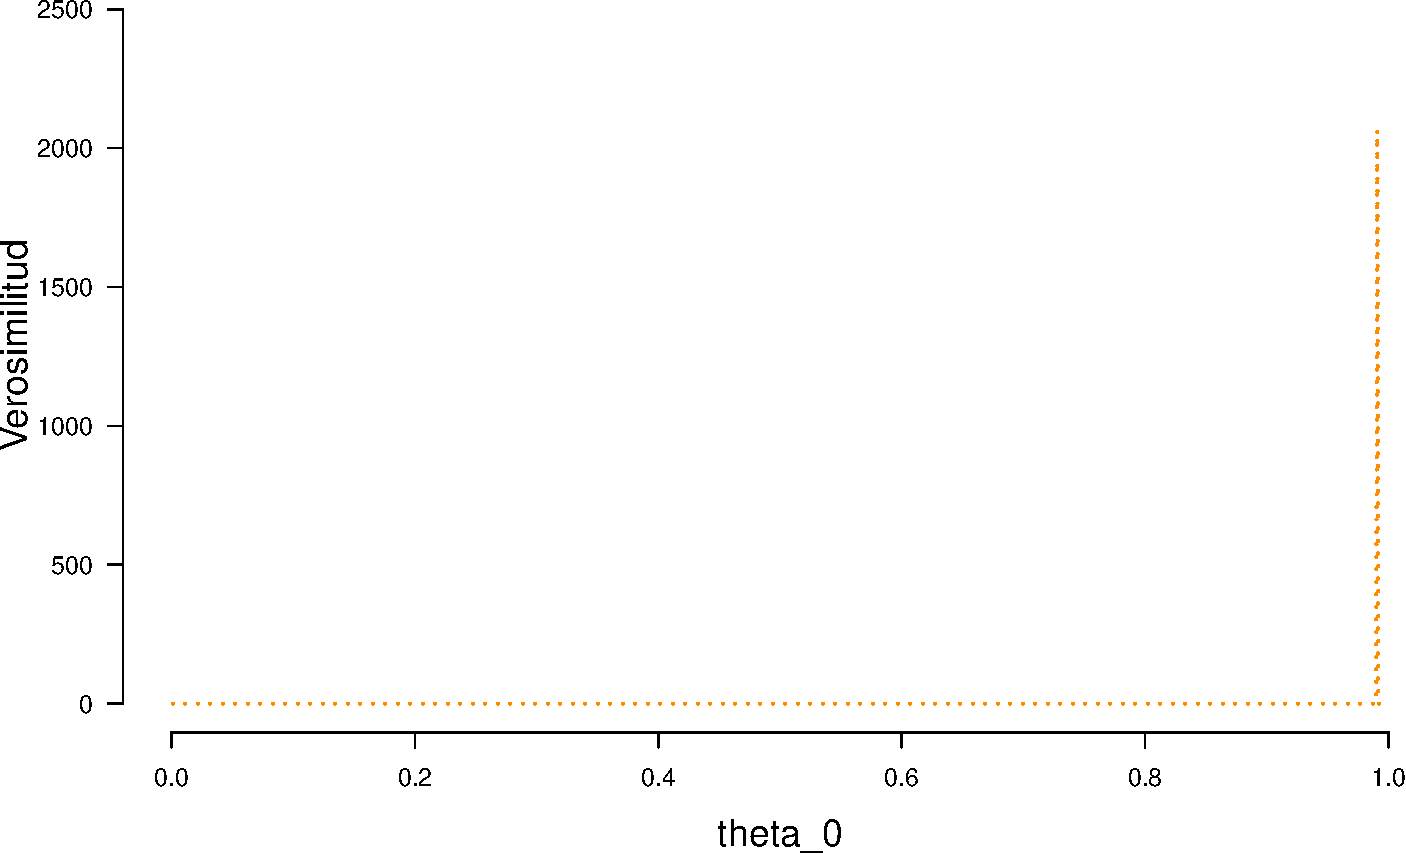
\includegraphics{act11302_sesion_03_files/figure-beamer/likelihhod-1.pdf}

\end{frame}

\begin{frame}{Reflexion}
\protect\hypertarget{reflexion}{}

\begin{itemize}
\tightlist
\item
  Aunque pareciera ser contundente, ?`es conveniente considerar
  solamente la informacion de estos ``datos''?
\end{itemize}

\end{frame}

\begin{frame}{Informacion complementaria}
\protect\hypertarget{informacion-complementaria}{}

Pensemos el caso en que informacion del siguiente tipo es disponible:

\begin{itemize}
\item
  (A). Creemos que la mediana de la incidencia de siniestros es
  \(0.85\).
\item
  (B). Creemos que el \(99.999\)-esimo porcentil de la incidencia de
  siniestros es \(0.95\).
\item
  (C). Creemos que el porcentil \(0.001\) de la incidencia de siniestros
  es \(0.60\).
\end{itemize}

\textcolor{blue}{Esta informacion complementaria resume la informacion de expertos / instituciones reguladoras / mercado / etc.}

\end{frame}

\begin{frame}[fragile]{Visualizacion de elicitacion}
\protect\hypertarget{visualizacion-de-elicitacion}{}

\begin{verbatim}
## [1] "Elicitacion para a= 52.22 b= 9.52105105105105"
\end{verbatim}

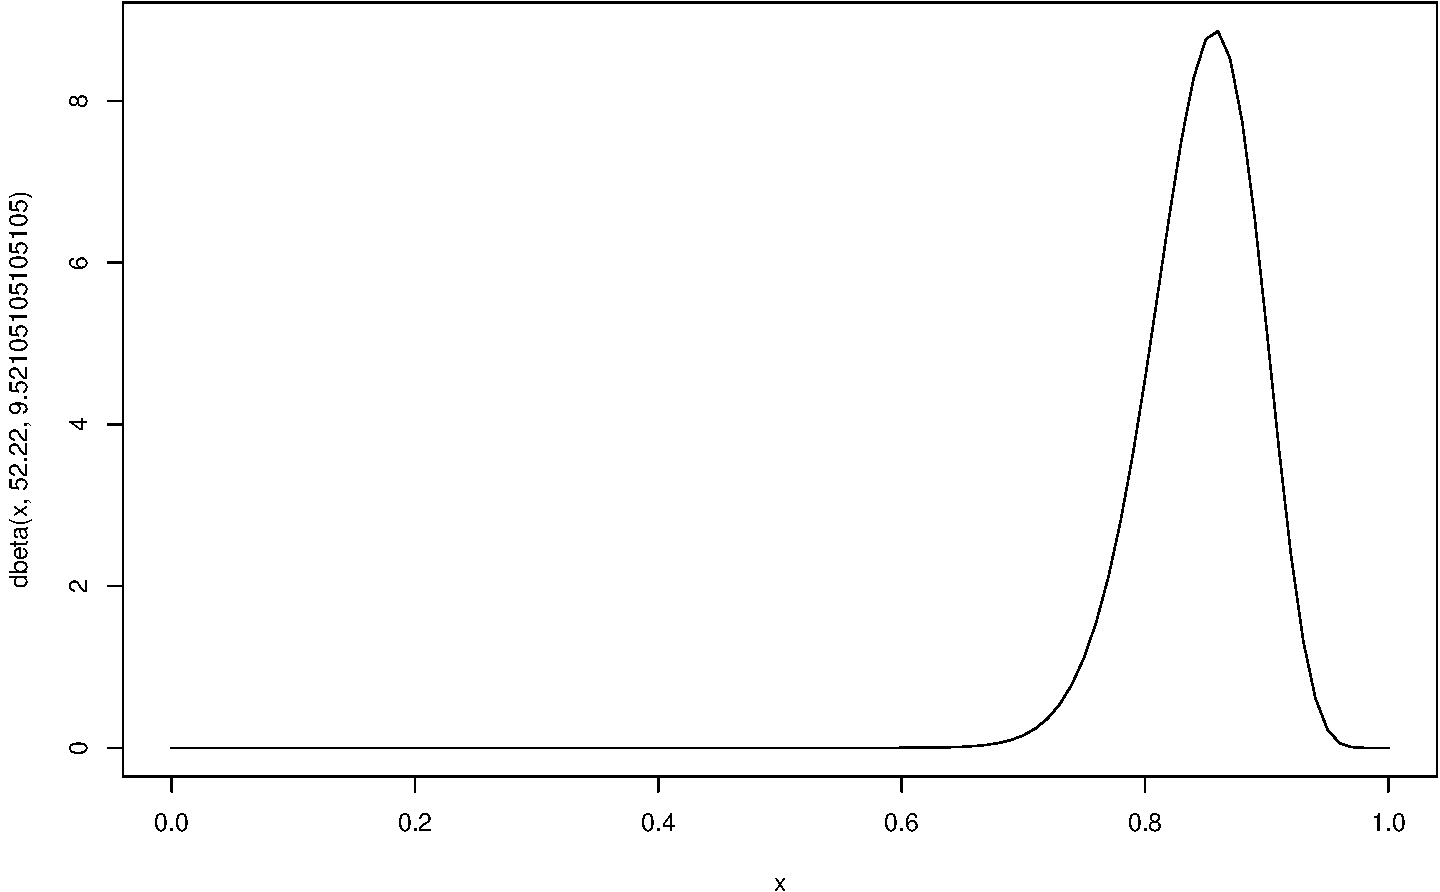
\includegraphics{act11302_sesion_03_files/figure-beamer/betaelicitacion-1.pdf}

\end{frame}

\begin{frame}[fragile]{Consolidacion de informacion}
\protect\hypertarget{consolidacion-de-informacion}{}

La informacion contenida en los \texttt{datos} y \texttt{complementaria}
se \textbf{consolida} en la siguiente expresion \[
q(\theta_0|\text{datos},\text{complemento}) \propto lik(\theta_0|\text{datos}) \times q(\theta_0|\text{complemento}).
\]

Resulta ser que si \(q(\theta_0|\text{complemento})\) es una medida de
probabilidad, la funcion \(q(\theta_0|\text{datos},\text{complemento})\)
tambien lo es.

En este caso, tal condicion se cumple, pues
\(q(\theta_0|\text{complemento})\) se elicito siendo parte de la familia
de distribuciones beta.

La funcion \(q(\theta_0|\text{complemento})\) se refiere a la
\textbf{prior} del modelo en el contexto bayesiano de inferencia.

\end{frame}

\begin{frame}[fragile]{Visualizacion de consolidacion}
\protect\hypertarget{visualizacion-de-consolidacion}{}

\begin{Shaded}
\begin{Highlighting}[]
\KeywordTok{consolidacion.binomialbeta}\NormalTok{(n0, J, }\FloatTok{52.22}\NormalTok{, }\FloatTok{9.52}\NormalTok{,}\DataTypeTok{print=}\OtherTok{TRUE}\NormalTok{,}\DataTypeTok{summary=}\OtherTok{FALSE}\NormalTok{)}
\end{Highlighting}
\end{Shaded}

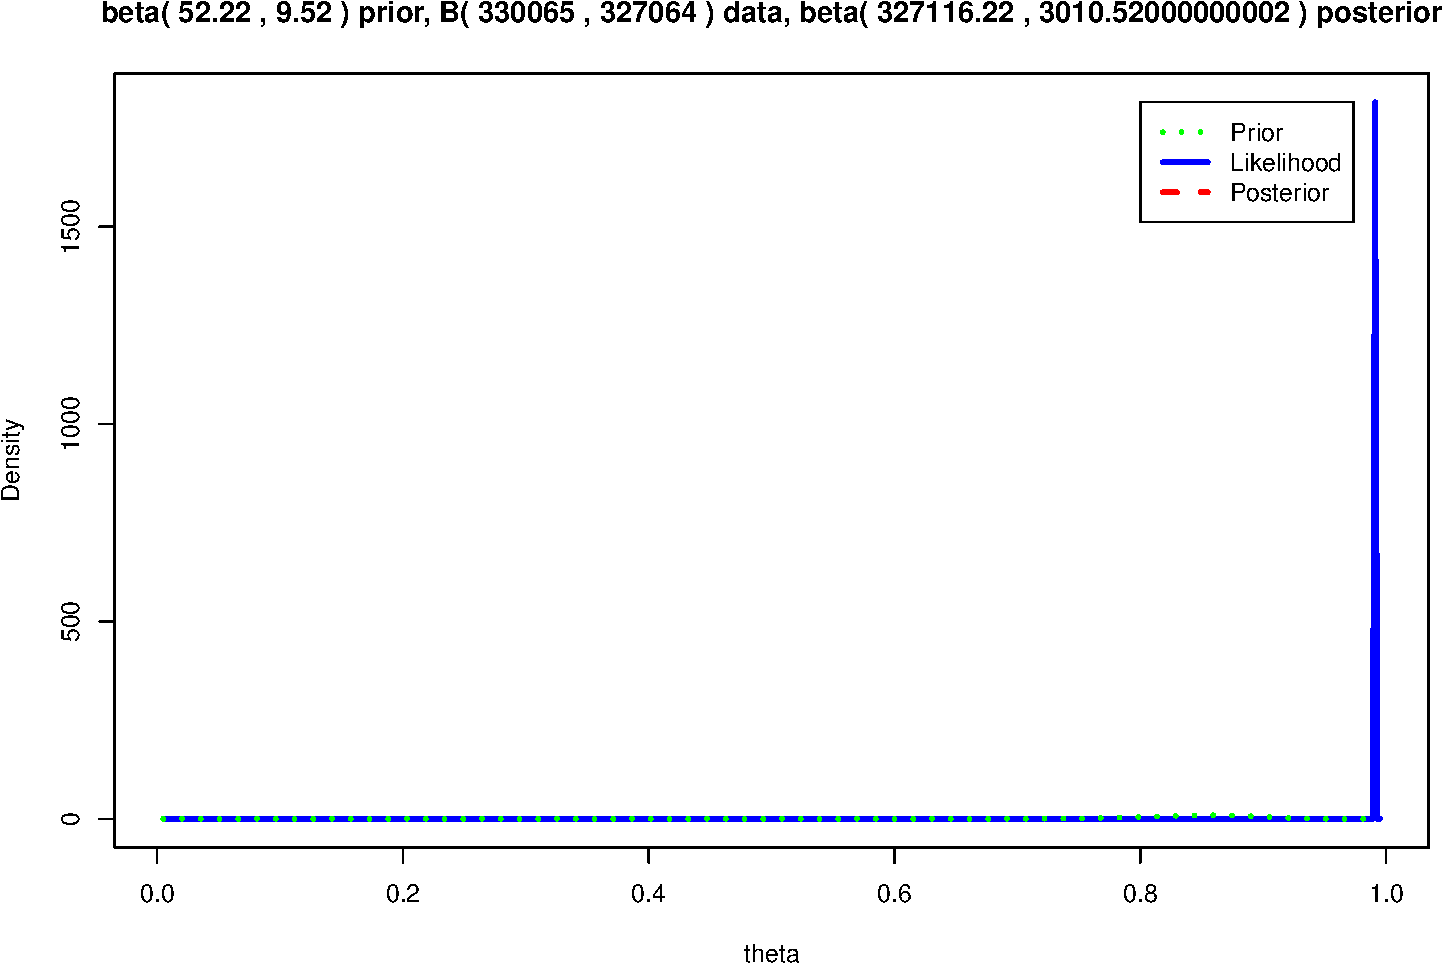
\includegraphics{act11302_sesion_03_files/figure-beamer/unnamed-chunk-2-1.pdf}

\end{frame}

\begin{frame}[fragile]{Error epistemico II}
\protect\hypertarget{error-epistemico-ii}{}

\begin{Shaded}
\begin{Highlighting}[]
\KeywordTok{consolidacion.binomialbeta}\NormalTok{(n0, J, }\FloatTok{52.22}\NormalTok{, }\FloatTok{9.52}\NormalTok{,}\DataTypeTok{print=}\OtherTok{FALSE}\NormalTok{,}\DataTypeTok{summary=}\OtherTok{TRUE}\NormalTok{)}
\end{Highlighting}
\end{Shaded}

\begin{verbatim}
## [1] "Modas= 0.857381988617342  |  0.990907851483799  |  0.990883688390031"
## [1] "Medias= 0.845804988662132  |  0.990904876888632  |  0.990880714479536"
## [1] "sd s= 0.0455929848904483  |  0.000165241284816415  |  0.000165443643283756"
\end{verbatim}

\end{frame}

\begin{frame}[fragile]{Ejercicio}
\protect\hypertarget{ejercicio}{}

\begin{enumerate}
\item
  Seleccionen una submuestra aleatoria del 10\% de los \texttt{datos}.
\item
  Replique los calculos usando los datos de la submuestra aleatoria.
\item
  Reflexione acerca de los \textbf{estimadores puntuales}, el
  \textbf{error epistemico} y relevancia de la \textbf{informacion
  complementaria}.
\end{enumerate}

\end{frame}


\section[]{}
\frame{\small \frametitle{Table of Contents}
\tableofcontents}
\end{document}
